
\begin{frame}{Various Tips}
  \begin{center}
    
\includegraphics[height=4cm]{img/linkedin.png}
  \end{center}
\end{frame}

\begin{frame}{Various Tips}
  \begin{block}{LinkedIn: Extreme Productivity}
    \begin{itemize}
      \item Use deadlines.
      \item Limit your perfectionism.
      \item Write/communicate with efficiency.
    \end{itemize}
  \end{block}
\end{frame}

\begin{frame}{Various Tips}
  \begin{block}{LinkedIn: Effective Listening}
    \begin{itemize}
      \item Roles of listeners. % listen for information or just to support/hear
      \item Big pictures vs. details.
      \item Paraphrase what was said. % you show you understand, you give yourself time
    \end{itemize}
  \end{block}
\end{frame}

\begin{frame}{Various Tips}
  \begin{block}{LinkedIn: Managing Your Energy}
    \begin{itemize}
      \item Personal body clock. Prime and low times.
      \item Pair your tasks with energy-required labels. 
    \end{itemize}
  \end{block}
\end{frame}

\begin{frame}{Various Tips}
  \begin{block}{LinkedIn: Prioritizing at Work}
    \begin{itemize}
      \item 3 questions.
      \item Magic question (= goal).
      \item What good shall I do today?
      \item What is my top priority today?
    \end{itemize}
  \end{block}
\end{frame}

\begin{frame}{Various Tips}
  \begin{block}{LinkedIn: The Six Morning Habits of High Performers}
    \begin{itemize}
      \item Silence, meditation.
      \item Affirmations, visualize to motivate yourself.
      \item Morning exercise. 
      \item Read. 
      \item Clarify your priorities.
      \item Appreciate (your current status).
    \end{itemize}
  \end{block}
\end{frame}

\begin{frame}{Various Tips}
  \begin{block}{LinkedIn: Enhancing Your Productivity}
    \begin{itemize}
      \item What makes you irreplacable?
      \item Spend most of your time doing most-valuable-activities.
      \item Avoid your least-valuable-activities.
    \end{itemize}
  \end{block}
\end{frame}

\begin{frame}{Various Tips}
  \begin{block}{LinkedIn: How to Slow Down and Be More Productive}
    \begin{itemize}
      \item Put breathing room in your schedule.
      \item Missing minute.
      \item Use minimal energy for maximum results (Pareto 80/20).
    \end{itemize}
  \end{block}
\end{frame}

\begin{frame}{Various Tips}
  \begin{block}{LinkedIn: Finding Your Productive Mindset}
    \begin{itemize}
      \item Make a not-todo list.
    \end{itemize}
  \end{block}
\end{frame}

\begin{frame}{Various Tips}
  \begin{block}{LinkedIn: 5S Workplace Productivity}
    \begin{itemize}
      \item Seiri/sort: remove all unnecessary things.
      \item Seiton/set in order: everything has its home, put it there.
      \item Seisou/shine: maintenance, inspect your tools regularly.
      \item Seiketsu/standardize: schedule and repeat first 3S.
      \item Shitsuke/sustain: self-discipline, do without being told.
    \end{itemize}
  \end{block}
\end{frame}

\begin{frame}{Various Tips}
  \begin{block}{LinkedIn: Be More Productive: Take Small Steps, Have Big Goals}
    \begin{itemize}
      \item Baby steps. 
    \end{itemize}
  \end{block}
\end{frame}

\begin{frame}{Various Tips}
  \begin{center}
    
\includegraphics[height=4cm]{img/others.png}
  \end{center}
\end{frame}

\begin{frame}{Various Tips}
  \begin{block}{Productivity habits I: https://fastertomaster.com}
    \begin{itemize}
      \item I get at least 7 to 8 hours of sleep.
      \item I wake up at the same time each day.
      \item I exercise at moderate/high intensity 3 to 4 days per week.
      \item I stay well hydrated throughout the day.
      \item I stick to a healthy, balanced and nutritious diet.
      \item I start my day with a streamlined and consistent morning routine.
      \item I work from a simple, prioritised, daily to-do list.
    \end{itemize}
  \end{block}
\end{frame}

\begin{frame}{Various Tips}
  \begin{block}{Productivity habits II: https://fastertomaster.com}
    \begin{itemize}
      \item I use journalling to clear my head and solve tricky problems.
      \item I spend at least 20 minutes per day in meditation or prayer.
      \item I regularly check in with my sensations, thoughts and emotions during the day.
      \item I get 3 or more hours of deep, purposeful work done each day.
      \item My various inboxes (including email) are under control and well organised.
      \item I have a clear, structured calendar system.
    \end{itemize}
  \end{block}
\end{frame}

\begin{frame}{Various Tips}
  \begin{block}{Productivity habits III: https://fastertomaster.com}
    \begin{itemize}
      \item I have a single, up-to-date list of all my doable next actions.
      \item I have a single list of all my active, 3 to 12-month projects.
      \item I check in with my written big-picture vision and mission statements.
      \item My folder and filing system is clear, current and well organised.
      \item I end each day with a streamlined and consistent evening routine.
      \item I know exactly where my time goes each day.
    \end{itemize}
  \end{block}
\end{frame}

\begin{frame}{Various Tips}
  \begin{block}{Productivity habits IV: https://fastertomaster.com}
    \begin{itemize}
      \item I'm actively working on and tracking a handful of habits.
      \item I finish each day with a clear plan for tomorrow. 
      \item I reflect on my wins, lessons and opportunities each day.
      \item I write down at least three things I’m grateful for each day.
      \item I make time each week to get clear, get current and reflect on the last 7 days.
      \item I make time each week to plan and set the next 7 days up for success.
    \end{itemize}
  \end{block}
\end{frame}

\begin{frame}{Various Tips}
  \begin{block}{Energy: https://theenergyproject.com/}
    \begin{itemize}
      \item Work on todo items based on your energy.
      \item Mark them as red ("energy required") and black ("easy").
    \end{itemize}
  \end{block}
\end{frame}

\begin{frame}{Various Tips}
  \begin{block}{Energy: https://theenergyproject.com/}
    \begin{center}
      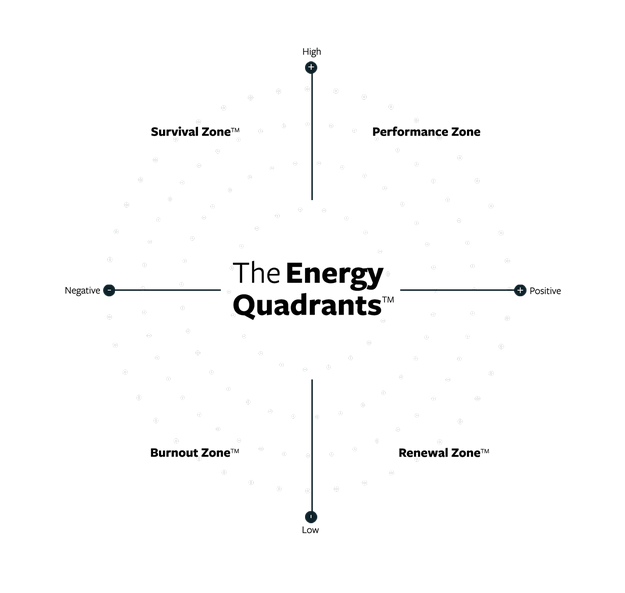
\includegraphics[height=6cm]{img/the-energy-project.png}
    \end{center}
  \end{block}
\end{frame}

\begin{frame}{Various Tips}
  \begin{block}{The Miracle Morning: https://niklasgoeke.com/the-miracle-morning/}
    \begin{itemize}
      \item Reading.
      \item Exercise.
      \item Affirmations.
      \item Silence.
      \item Visualization.
      \item Scribing/journaling.
      \item Doing your Most Important Thing.
    \end{itemize}
  \end{block}
\end{frame}

\begin{frame}{Various Tips}
  \begin{block}{From others}
    \begin{itemize}
      \item Go to cafe without WIFI/password.
      \item Give yourself a treat after work.
      \item Use a specific place just for work.
      \item Hit more birds with one stone (kill 2 flies with one hit).
      \item US study with focus, 25-30m, a girl studying 4h each night.
      \item 30m work + 5m rest.
    \end{itemize}
  \end{block}
\end{frame}

\begin{frame}{Various Tips}
  \begin{block}{My experience}
    \begin{itemize}
      \item Pomodoro did not work well. % ending a block just before finishing a task, having time left, meetings, ...
      \item GTD: phone, calendar, door, trello, online sheet. No regular reviews.
      \item 30 minutes a day!
      \item Start slow, make baby steps. % my books reading, hand-stand
      \item (Intermittent) fasting clears your mind and senses. No feeling-down after lunch.
      \item Regular exercise.
      \item My school studying in a train station waiting room.
    \end{itemize}
  \end{block}
\end{frame}

